\documentclass[a4paper, oneside, final]{memoir}
\usepackage[T1]{fontenc}
\usepackage[utf8]{inputenc}
\usepackage[british]{babel}
\usepackage{amsmath}
\usepackage{amsthm}
\usepackage{ifthen}
\usepackage{verbatim}

% bedre orddeling Gør at der som minimum skal blive to tegn på linien ved
% orddeling og minimum flyttes to tegn ned på næste linie. Desværre er værdien
% anvendt af babel »12«, hvilket kan give orddelingen »h-vor«.
\renewcommand{\britishhyphenmins}{22} 

% Fix of fancyref to work with memoir. Makes references look
% nice. Redefines memoir \fref and \Fref to \refer and \Refer.
% \usepackage{refer}             %
% As we dont really have any use for \fref and \Fref we just undefine what
% memoir defined them as, so fancyref can define what it wants.
\let\fref\undefined
\let\Fref\undefined
\usepackage{fancyref} % Better reference. 

\usepackage{pdflscape} % Gør landscape-environmentet tilgængeligt
\usepackage{fixme}     % Indsæt "fixme" noter i drafts.
\usepackage{hyperref}  % Indsæter links (interne og eksterne) i PDF

\usepackage[format=hang]{caption,subfig}
\usepackage{graphicx}
\usepackage{stmaryrd}
\usepackage{amssymb}
\usepackage{listings}
\usepackage{ulem} % \sout - strike-through
\usepackage{tikz}

%\renewcommand{\ttdefault}{txtt} % Bedre typewriter font
% \usepackage[sc]{mathpazo}     % Palatino font
%\renewcommand{\rmdefault}{urw-garamond} % Garamond
%\usepackage[urw-garamond]{mathdesign}

% \overfullrule=5pt
% \setsecnumdepth{part}
\setcounter{secnumdepth}{1} % Sæt overskriftsnummereringsdybde. Disable = -1.
\setlength{\parskip}{0.25in}

\title{Statistical Methods for Machine Learning\\Case 1}

\author{Troels Henriksen (athas@sigkill.dk) \\ Daniel Fairchild
  (daniel.fairchild@gmail.com)}

\date{\today}
\pagestyle{plain}

\newcommand{\nfrac}[2]{\frac{\displaystyle{#1}}{\displaystyle{#2}}}

\newcommand{\cninesmean}{\[\begin{pmatrix}
 244.482118 & 76.670747 & 65.978559 \\
\end{pmatrix}\]}

\newcommand{\cninescov}{\[\begin{pmatrix}
 455.554503 & 317.875048 & 406.207404 \\
 317.875048 & 1118.698163 & 1300.346182 \\
 406.207404 & 1300.346182 & 1573.115002 \\
\end{pmatrix}\]}


\newcommand{\ctensmean}{\[\begin{pmatrix}
 244.482118 & 76.670747 & 65.978559 \\
\end{pmatrix}\]}

\newcommand{\ctenscov}{\[\begin{pmatrix}
 455.554503 & 317.875048 & 406.207404 \\
 317.875048 & 1118.698163 & 1300.346182 \\
 406.207404 & 1300.346182 & 1573.115002 \\
\end{pmatrix}\]}

\newcommand{\ctenwmean}{\[\begin{pmatrix}
 236.669843 & 302.225900 \\
\end{pmatrix}\]}

\newcommand{\ctenwcov}{\[\begin{pmatrix}
 2743.075724 & -217.633352 \\
 -217.633352 & 8723.156267 \\
\end{pmatrix}\]}


\newcommand{\celevenwmean}{\[\begin{pmatrix}
 175.982719 & 194.933287 \\
\end{pmatrix}\]}

\newcommand{\celevenwcov}{\[\begin{pmatrix}
 2335.395665 & -197.732010 \\
 -197.732010 & 1688.149233 \\
\end{pmatrix}\]}



\begin{document}

\maketitle

We have never used R before, so for the novelty, that is the language
we have decided to use for this assignment.

\section*{Question 1.1}

The following plot has been produced through straightforward use of
the \texttt{dnorm} function and plotting facilities in R.  A thousand
sample points have been used.  The code for this question is in the
file \texttt{question11.R}.

\begin{figure}
 \begin{centering}
    % GNUPLOT: LaTeX picture with Postscript
\begingroup
  \makeatletter
  \providecommand\color[2][]{%
    \GenericError{(gnuplot) \space\space\space\@spaces}{%
      Package color not loaded in conjunction with
      terminal option `colourtext'%
    }{See the gnuplot documentation for explanation.%
    }{Either use 'blacktext' in gnuplot or load the package
      color.sty in LaTeX.}%
    \renewcommand\color[2][]{}%
  }%
  \providecommand\includegraphics[2][]{%
    \GenericError{(gnuplot) \space\space\space\@spaces}{%
      Package graphicx or graphics not loaded%
    }{See the gnuplot documentation for explanation.%
    }{The gnuplot epslatex terminal needs graphicx.sty or graphics.sty.}%
    \renewcommand\includegraphics[2][]{}%
  }%
  \providecommand\rotatebox[2]{#2}%
  \@ifundefined{ifGPcolor}{%
    \newif\ifGPcolor
    \GPcolortrue
  }{}%
  \@ifundefined{ifGPblacktext}{%
    \newif\ifGPblacktext
    \GPblacktextfalse
  }{}%
  % define a \g@addto@macro without @ in the name:
  \let\gplgaddtomacro\g@addto@macro
  % define empty templates for all commands taking text:
  \gdef\gplbacktext{}%
  \gdef\gplfronttext{}%
  \makeatother
  \ifGPblacktext
    % no textcolor at all
    \def\colorrgb#1{}%
    \def\colorgray#1{}%
  \else
    % gray or color?
    \ifGPcolor
      \def\colorrgb#1{\color[rgb]{#1}}%
      \def\colorgray#1{\color[gray]{#1}}%
      \expandafter\def\csname LTw\endcsname{\color{white}}%
      \expandafter\def\csname LTb\endcsname{\color{black}}%
      \expandafter\def\csname LTa\endcsname{\color{black}}%
      \expandafter\def\csname LT0\endcsname{\color[rgb]{1,0,0}}%
      \expandafter\def\csname LT1\endcsname{\color[rgb]{0,1,0}}%
      \expandafter\def\csname LT2\endcsname{\color[rgb]{0,0,1}}%
      \expandafter\def\csname LT3\endcsname{\color[rgb]{1,0,1}}%
      \expandafter\def\csname LT4\endcsname{\color[rgb]{0,1,1}}%
      \expandafter\def\csname LT5\endcsname{\color[rgb]{1,1,0}}%
      \expandafter\def\csname LT6\endcsname{\color[rgb]{0,0,0}}%
      \expandafter\def\csname LT7\endcsname{\color[rgb]{1,0.3,0}}%
      \expandafter\def\csname LT8\endcsname{\color[rgb]{0.5,0.5,0.5}}%
    \else
      % gray
      \def\colorrgb#1{\color{black}}%
      \def\colorgray#1{\color[gray]{#1}}%
      \expandafter\def\csname LTw\endcsname{\color{white}}%
      \expandafter\def\csname LTb\endcsname{\color{black}}%
      \expandafter\def\csname LTa\endcsname{\color{black}}%
      \expandafter\def\csname LT0\endcsname{\color{black}}%
      \expandafter\def\csname LT1\endcsname{\color{black}}%
      \expandafter\def\csname LT2\endcsname{\color{black}}%
      \expandafter\def\csname LT3\endcsname{\color{black}}%
      \expandafter\def\csname LT4\endcsname{\color{black}}%
      \expandafter\def\csname LT5\endcsname{\color{black}}%
      \expandafter\def\csname LT6\endcsname{\color{black}}%
      \expandafter\def\csname LT7\endcsname{\color{black}}%
      \expandafter\def\csname LT8\endcsname{\color{black}}%
    \fi
  \fi
  \setlength{\unitlength}{0.0500bp}%
  \begin{picture}(7200.00,5040.00)%
    \gplgaddtomacro\gplbacktext{%
      \csname LTb\endcsname%
      \put(1078,704){\makebox(0,0)[r]{\strut{} 0}}%
      \put(1078,1168){\makebox(0,0)[r]{\strut{} 0.05}}%
      \put(1078,1632){\makebox(0,0)[r]{\strut{} 0.1}}%
      \put(1078,2096){\makebox(0,0)[r]{\strut{} 0.15}}%
      \put(1078,2559){\makebox(0,0)[r]{\strut{} 0.2}}%
      \put(1078,3023){\makebox(0,0)[r]{\strut{} 0.25}}%
      \put(1078,3487){\makebox(0,0)[r]{\strut{} 0.3}}%
      \put(1078,3951){\makebox(0,0)[r]{\strut{} 0.35}}%
      \put(1078,4415){\makebox(0,0)[r]{\strut{} 0.4}}%
      \put(2089,484){\makebox(0,0){\strut{}-5}}%
      \put(3246,484){\makebox(0,0){\strut{} 0}}%
      \put(4402,484){\makebox(0,0){\strut{} 5}}%
      \put(5559,484){\makebox(0,0){\strut{} 10}}%
      \put(6715,484){\makebox(0,0){\strut{} 15}}%
      \put(176,2739){\rotatebox{-270}{\makebox(0,0){\strut{}Y}}}%
      \put(4006,154){\makebox(0,0){\strut{}X}}%
    }%
    \gplgaddtomacro\gplfronttext{%
      \csname LTb\endcsname%
      \put(5816,4602){\makebox(0,0)[r]{\strut{}$\mu$=-1, $\sigma$=1}}%
      \csname LTb\endcsname%
      \put(5816,4382){\makebox(0,0)[r]{\strut{}$\mu$=2, $\sigma$=2}}%
      \csname LTb\endcsname%
      \put(5816,4162){\makebox(0,0)[r]{\strut{}$\mu$=3, $\sigma$=3}}%
    }%
    \gplbacktext
    \put(0,0){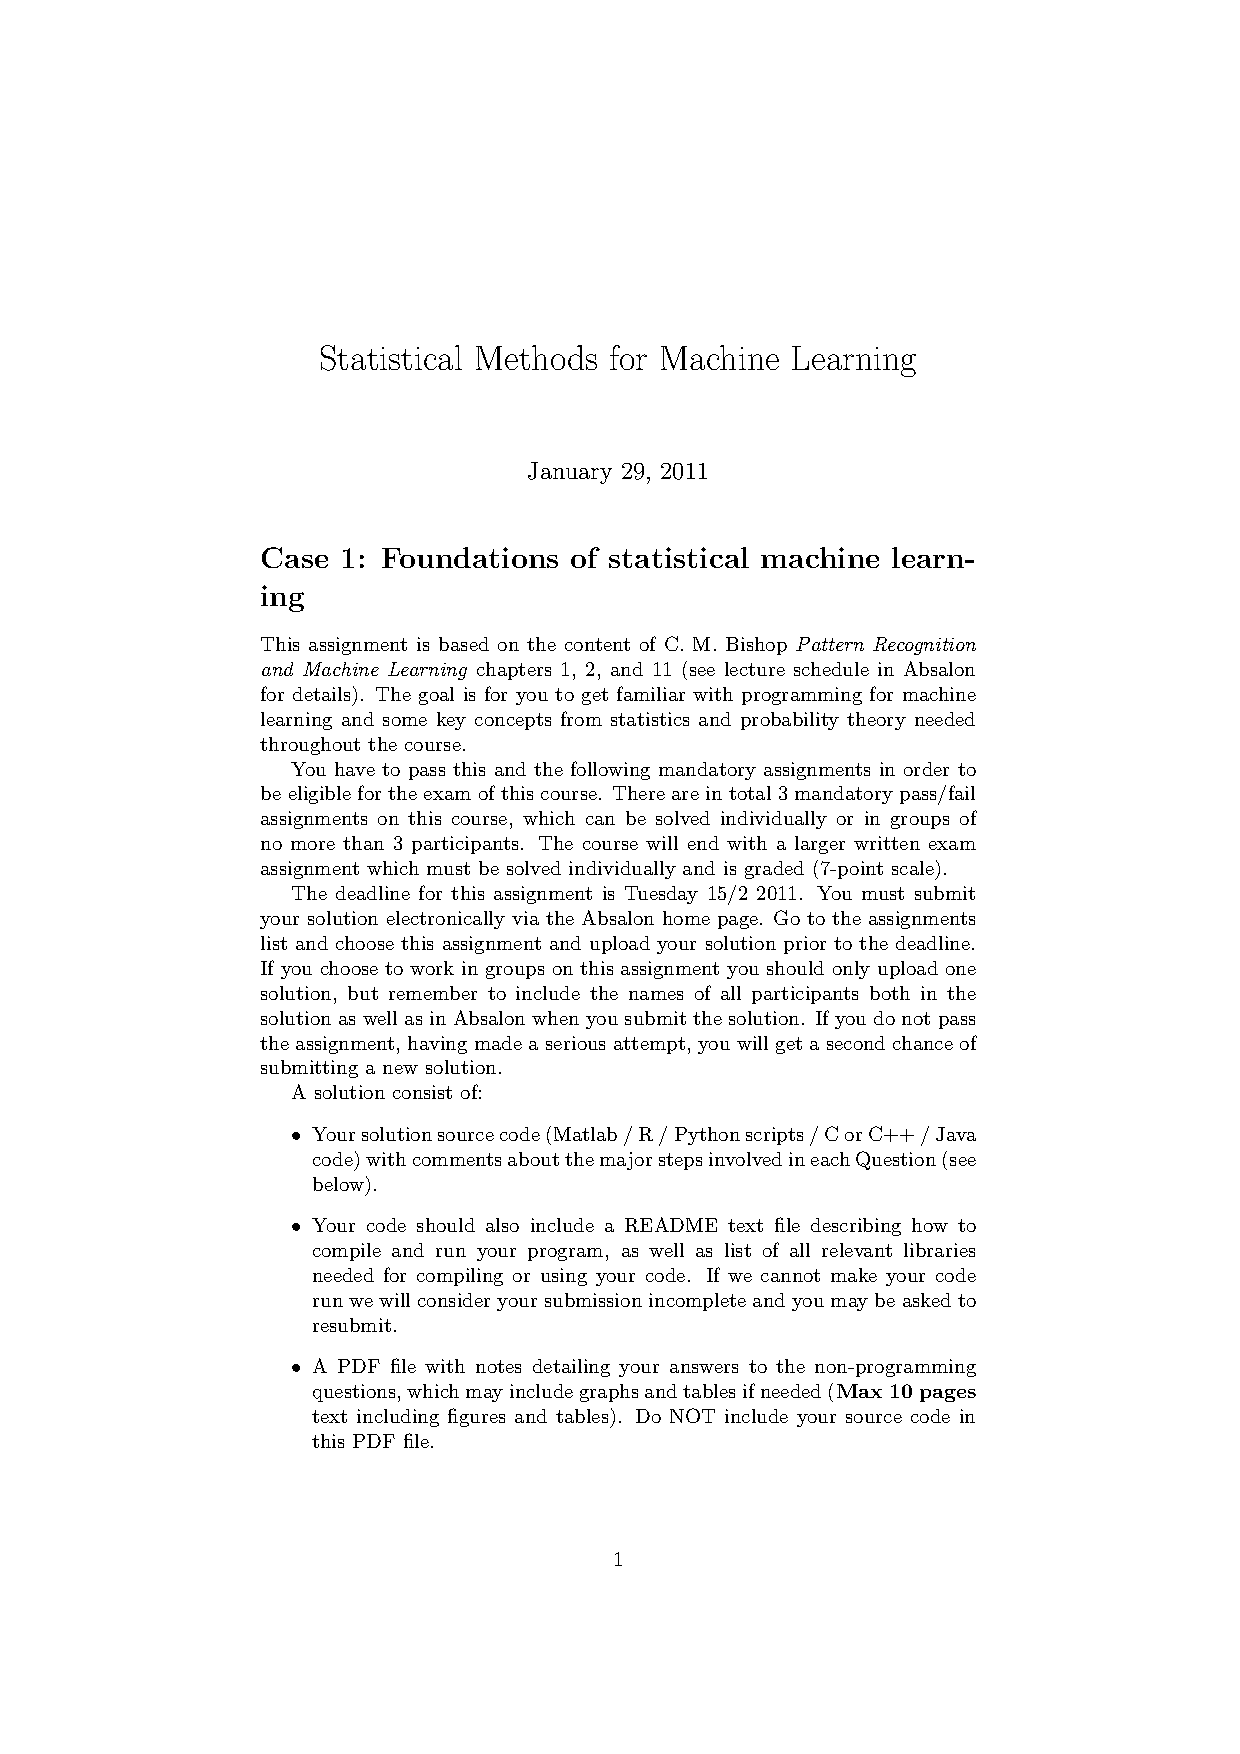
\includegraphics{tex_out/case1}}%
    \gplfronttext
  \end{picture}%
\endgroup

%  \label{foobar}
 \end{centering}
\end{figure}


\section*{Question 1.2}

The matrix
\[
M=\left[\begin{matrix}
  x_{1,1}&\cdots&x_{1,m}\\\vdots&\ddots&\vdots\\x_{n,1}&\cdots&x_{n,m} \end{matrix}\right]
\]
is \textit{positive definite} if for any nonzero real-entried vector
\[
V=\left[\begin{matrix} y_1 \\ \vdots \\ y_m \end{matrix}\right]
\]
we have
\[
V^TMV > 0.
\]

$M$ is \textit{symmetric} if $M^T=M$.

$M$ is \textit{square} if $m=n$.

An eigenvalue $\lambda$ is positive if $\lambda > 0$.

\section*{Question 1.3}

The code for this question is in the file \texttt{question131415.R}.

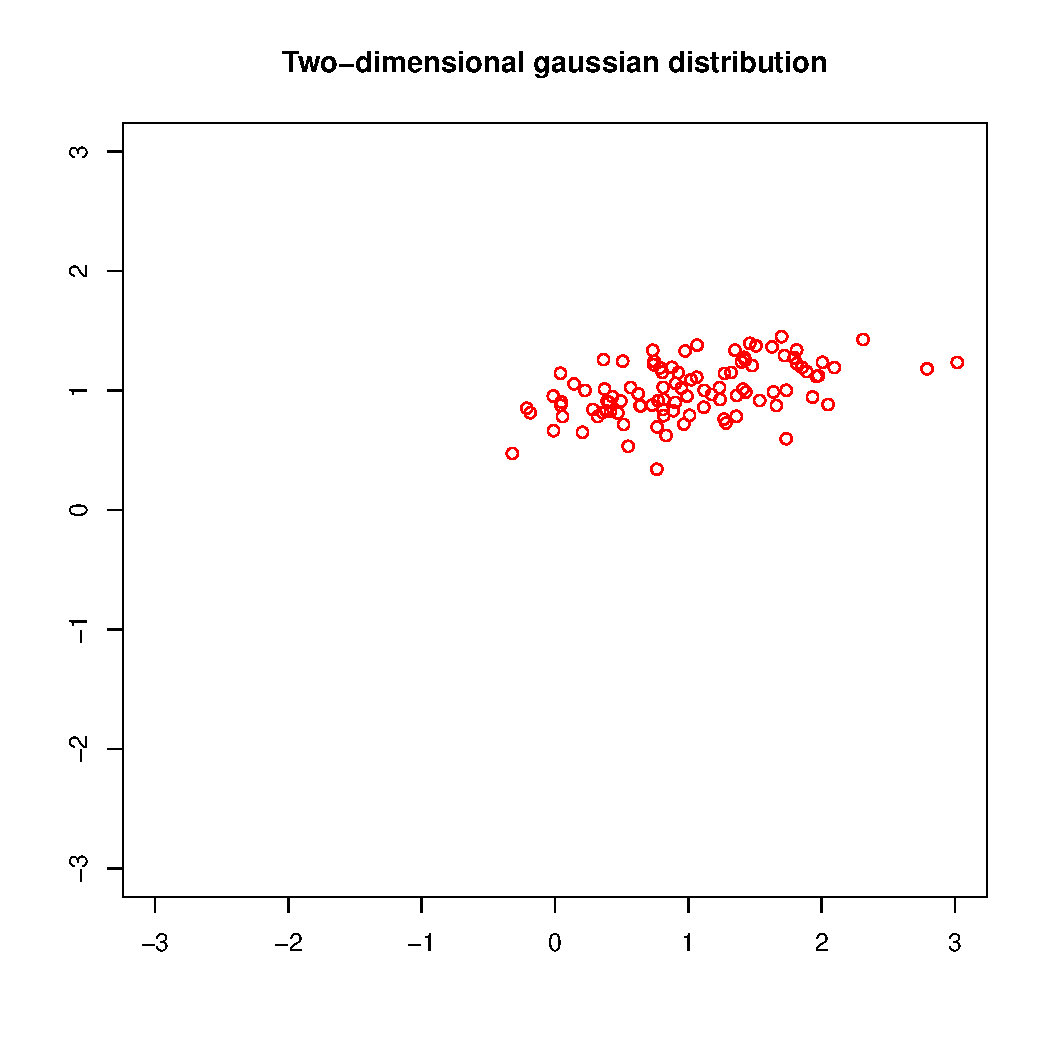
\includegraphics[width=10cm]{img/question13-plot.eps}

\section*{Question 1.4}

The code for this question is in the file \texttt{question131415.R}

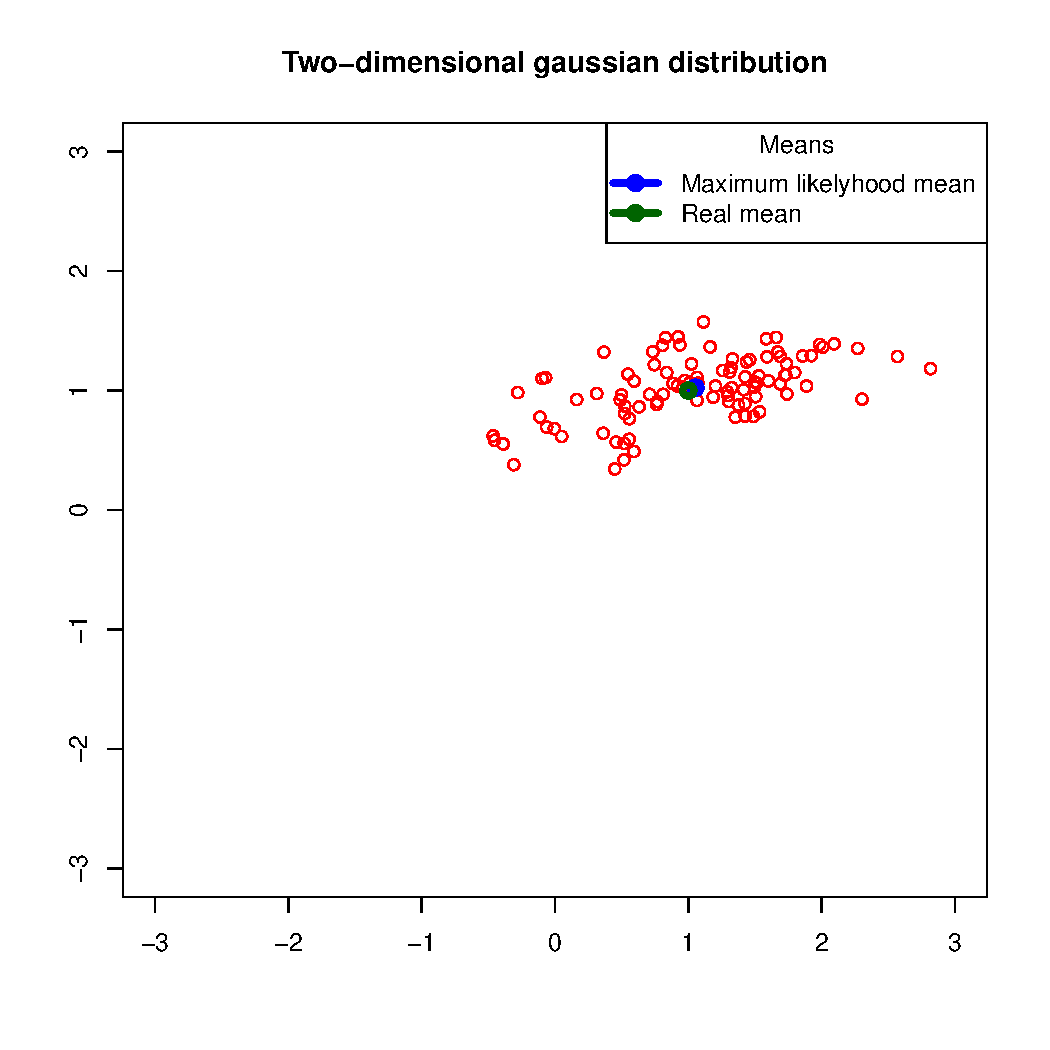
\includegraphics[width=10cm]{img/question14-plot.eps}

On a particular sampling the following sample covariance was observed
\[
\left[\begin{matrix}0.3085769&0.2101958\\0.2101958&0.2042408\end{matrix}\right]
\]
along with the sample mean
\[
\left[\begin{matrix}0.9855921\\0.9914642\end{matrix}\right]
\]

The Euclidian distance from the sample mean to the real mean is
\[
\sqrt{(0.9855921-1)^2+(0.9914642-1)^2}=0.01674
\]

This deviation could be due to the low number of samples.

\section*{Question 1.5}

The code for this question is in the file \texttt{question131415.R}.\\
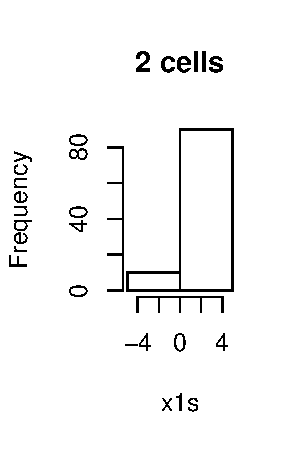
\includegraphics{img/question15-plot-1-a.eps}
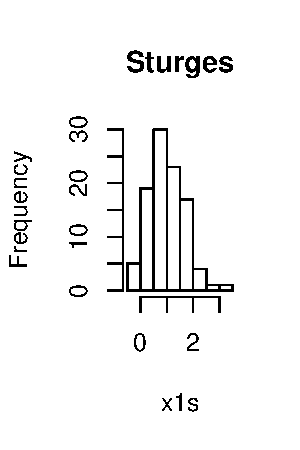
\includegraphics{img/question15-plot-1-b.eps}
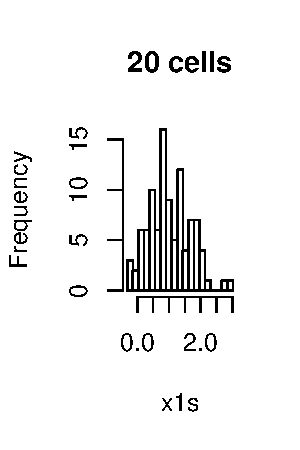
\includegraphics{img/question15-plot-1-c.eps}
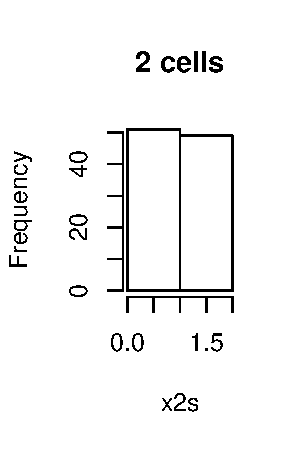
\includegraphics{img/question15-plot-2-a.eps}
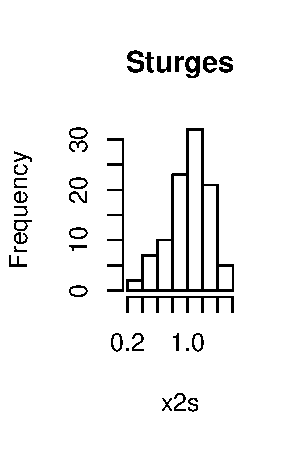
\includegraphics{img/question15-plot-2-b.eps}
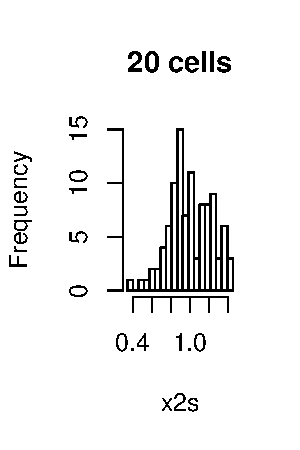
\includegraphics{img/question15-plot-2-c.eps}

As the bin width decreases, the random variation in the data results
in new local maximums that make the distribution appear more jagged
than it really is.

There is no best method to select bin widths, as the.  A common
method is Sturges' formula, where the $n$ data points are divided into
$\lceil\log_2n+1 \rceil$ bins.

\section*{Question 1.6}

The histogram is plotted with respect to density, rather than
frequency, so it can be easily compared to the density curve.  As can
be seen, the histogram with six bars fits the analytical curve well.

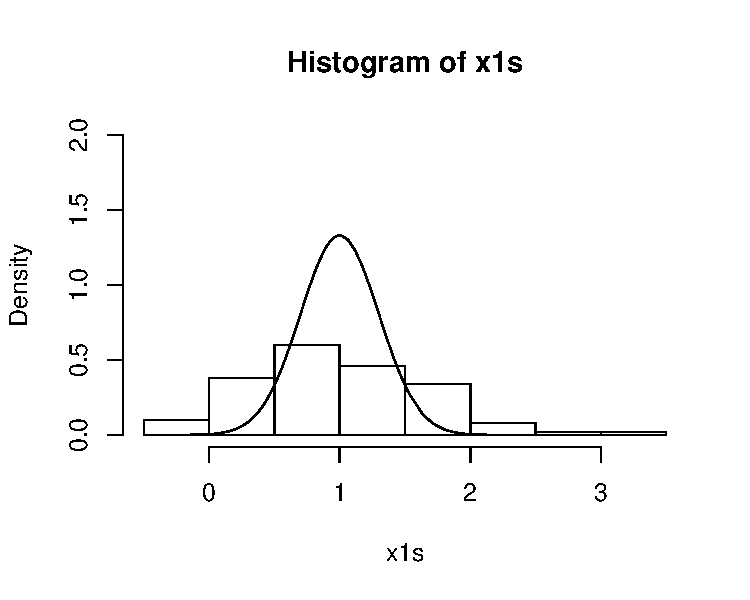
\includegraphics{img/question16-plot-analytical.eps}

The marginal distribution has the following analytical expression.

\begin{align*}
  p(x_1) &= \mathcal{N}(x_1|\mu_1,\Sigma_{1,1}) & \text{By CB (2.98)}\\
  &=
  \frac{1}{(2\pi\sigma_{1,1}^2)^{1/2}}\exp\left({-\frac{1}{2\sigma_{1,1}^2}(x_1-\mu_1)^2}\right)
  & \text{Substituting definition} \\
  &=
  \frac{1}{(2\pi\cdot 0.2^2)^{1/2}}\exp\left({-\frac{1}{2\cdot0.2^2}(x_1-1)^2}\right)
  & \text{Substituting $\sigma_{1,1}=0.2,\mu_1=1$}
\end{align*}

\section*{Question 1.7}

\includegraphics{img/question17-plot-100.eps}
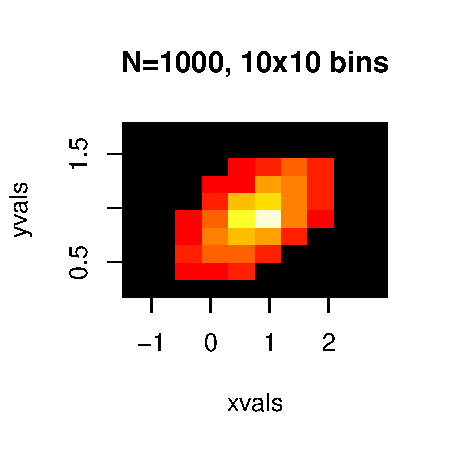
\includegraphics{img/question17-plot-1000-10x10.eps}
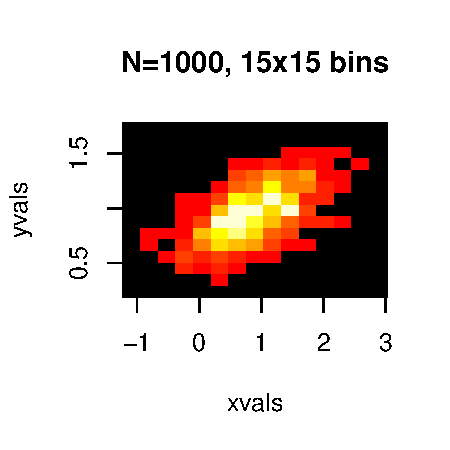
\includegraphics{img/question17-plot-1000-15x15.eps}
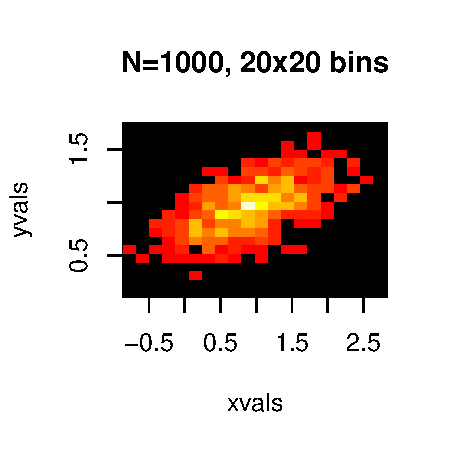
\includegraphics{img/question17-plot-1000-20x20.eps}
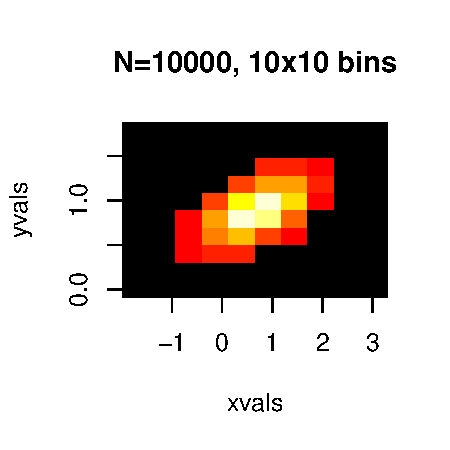
\includegraphics{img/question17-plot-10000.eps}

\section*{Question 1.8}


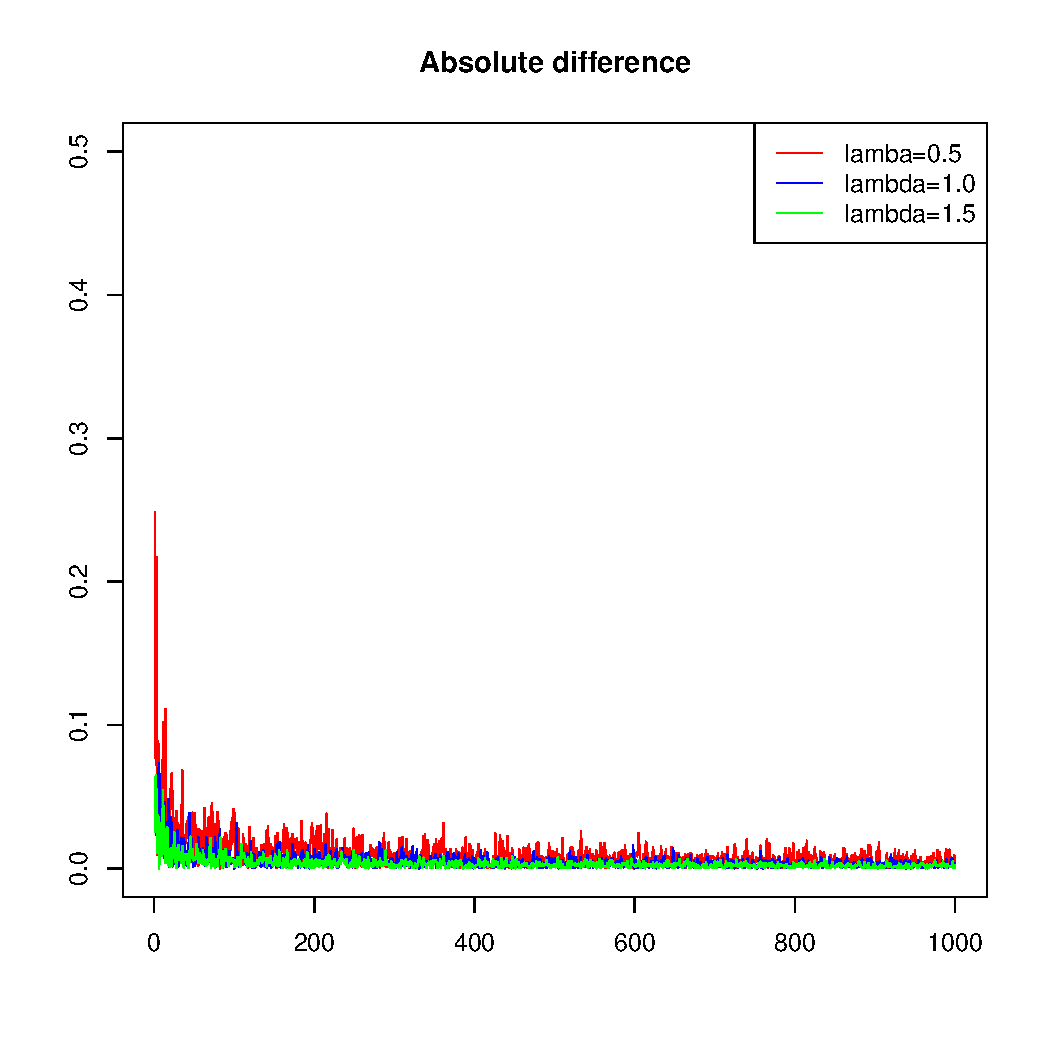
\includegraphics[width=10cm]{img/question18-plot-1.eps}

On a logarithmic $y$-axis, the plot above would consist of straight
lines.


\section*{Question 1.9}
From this question onwards we switched to coding in Ansi C. 

Our general purpose statml methods are gathered subfolder \textit{statml} and the more particular functions for the assignments at hand are to be found in the \textit{common case.h} and \textit{common case.c} files respectively.
PNM image format handling is provided by a custom library provided in the files \textit{pnm.h} and  \textit{pnm.c}.

The GSL library is required to compile all of the above and the gnuplot program is required to generate to iso-probability curves for questions 1.10 and 1.11.

Given that the above requirements are met, the three programs for subassignments 1.9, 1.10 and 1.11 should compile by writing \textit{make run\_all} in a shell.

Have a look at the source code in mycase9.c for the sequence of operations performed to generate the sample mean of:
\cninesmean{}
and the covariance of:
\cninescov{}
from the training set.

These are then used as input for the Probability Density Function, as given in the assignment, which is run on every pixel to generate a density map. The density map is normalized to $[0\cdots255]$ and output as the following grayscale image:
\begin{center}
\includegraphics[width=0.5\textwidth]{dimg/case9probmap1.pdf}
\end{center}
It can be seen from the image above that not all pixels of the pitcher are distinctly capture by this approach. The picture appears to have been taken with a flash, providing a uniform hue distribution across most of the pitcher. The exception are where the surface points most away from the camera, which have a darker hue of red.

\section*{Question 1.10}
The weighted average position is calculated from the probability density map with the formula given in the assignment with the result:
\ctenwmean{}
The weighted average position is then used to calculate the spatial covariance:
\ctenwcov{}
Our program generates two datafiles are then generated for plotting by gnuplot. One  contains a presentation of the background image and the other a probability density map generated from the weighted average position and spatial covariance given above. The file \textit{plot.gnu} is a gnuplot script that uses the two files mentioned above to generate the following image:

\includegraphics[width=0.8\textwidth]{tex_out/case10.pdf}
The iso-probability curves in the resulting plot seem to capture the distribution of "pitcher coloured" pixels in the given image. The weighted average position has been plotted as a green square and seems to be aligned correctly at the center of the iso-probability curves.

\section*{Question 1.11}
When applying our sample mean and covariance from kande1 on kande2, we get the following weighted average position:
\celevenwmean{}
and the following spatial covariance:
\celevenwcov{}
Plotting these as iso-probability curves on top of kande2 gives the following image:

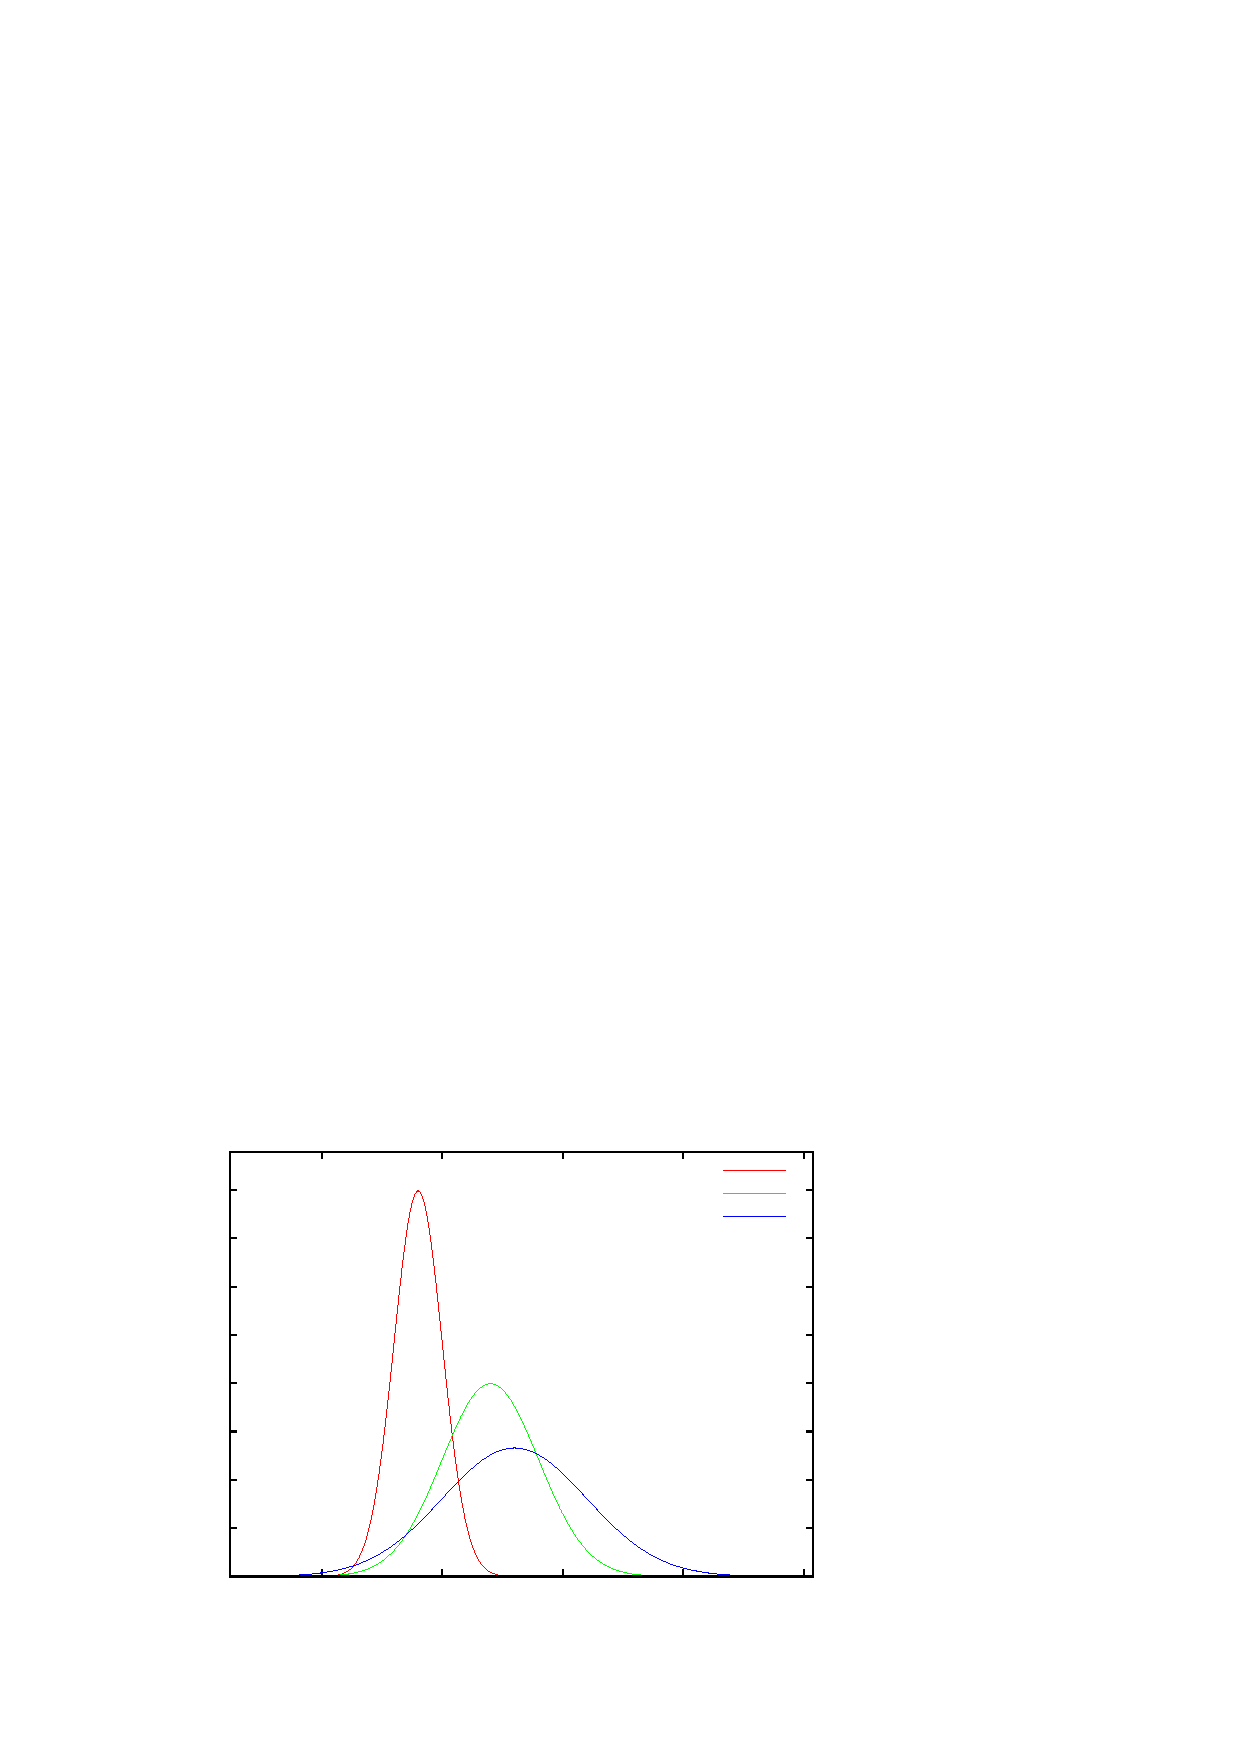
\includegraphics[width=0.8\textwidth]{tex_out/case11.pdf}

It is evident that the pitcher surface of kande2 is a lot less uniform than kande1, and it seems our model has recognized the collection of pixels with a similar colour distribution to that of the training set in kande1.

It seems that this approach is not able to reliably detect the outline of the red pitcher in the kande2 image with training data from the kande1 image.
\end{document}
